 %% 正文

\chapter{绪论}

\section{研究背景}
大容量、低成本、高性能的存储系统设计一直是存储领域研究的热点,而且随着大数据云存储时代的到来,人们
对这样的存储系统的要求更加迫切。而传统的磁盘虽然容量大价格低,但磁盘的机械特性导致了它的性能在很大
程度上已经到达极限。因此人们将希望寄托于新型的存储介质上,比如闪存存储器和相变存储器等。近年来固态
硬盘已经成为固态硬盘(SSD)已经成为固态技术中的领先技术,最常见的SSD都是基于NAND Flash芯片设计的。
SSD以闪存作为存储介质,具有随机读取速度快,功耗低,抗震性好等优点。因此目前广泛运用于家用和企业市场,
在发展中的云存储系统中渐渐取代了传统的普通机械硬盘。


但是,目前依然存在一些问题,比如在对数据安全性要求高的场合,普通的SSD组成的阵列无法保证数据的安全。
另外,由于SSD固有的特点,被删除的数据依旧可能被非法窃取,导致数据泄露等安全事故。针对这些存在的问题,
本研究旨在固态盘阵列存储系统之上设计一套冗余存储方案,存储的数据经过与其哈希信息复杂运算后,生成冗余
的加密数据,只要在物理意义上完全删除哈希信息或者一定量的数据块,原始数据即无法恢复,保证数据的安全。


固态盘的特性决定了,普通删除方式是根本不可能“真正”删除数据的,数据依然存在物理介质上\cite{ssd-outofplace-and-trim}。
在对闪存页(page)写操作时,需要首先进行块擦除操作,因此,不能对闪存进行就地更新(in-place-update)的操作,
只能采用异地更新(out-of-place update)的写方式,这就导致了旧的数据在某个时间窗口内依然存留在闪存上,删除
操作只是系统反馈的一个“假的”删除成功。数据删除整个过程如\autoref{fig:1}所示。
\begin{figure}
\centering
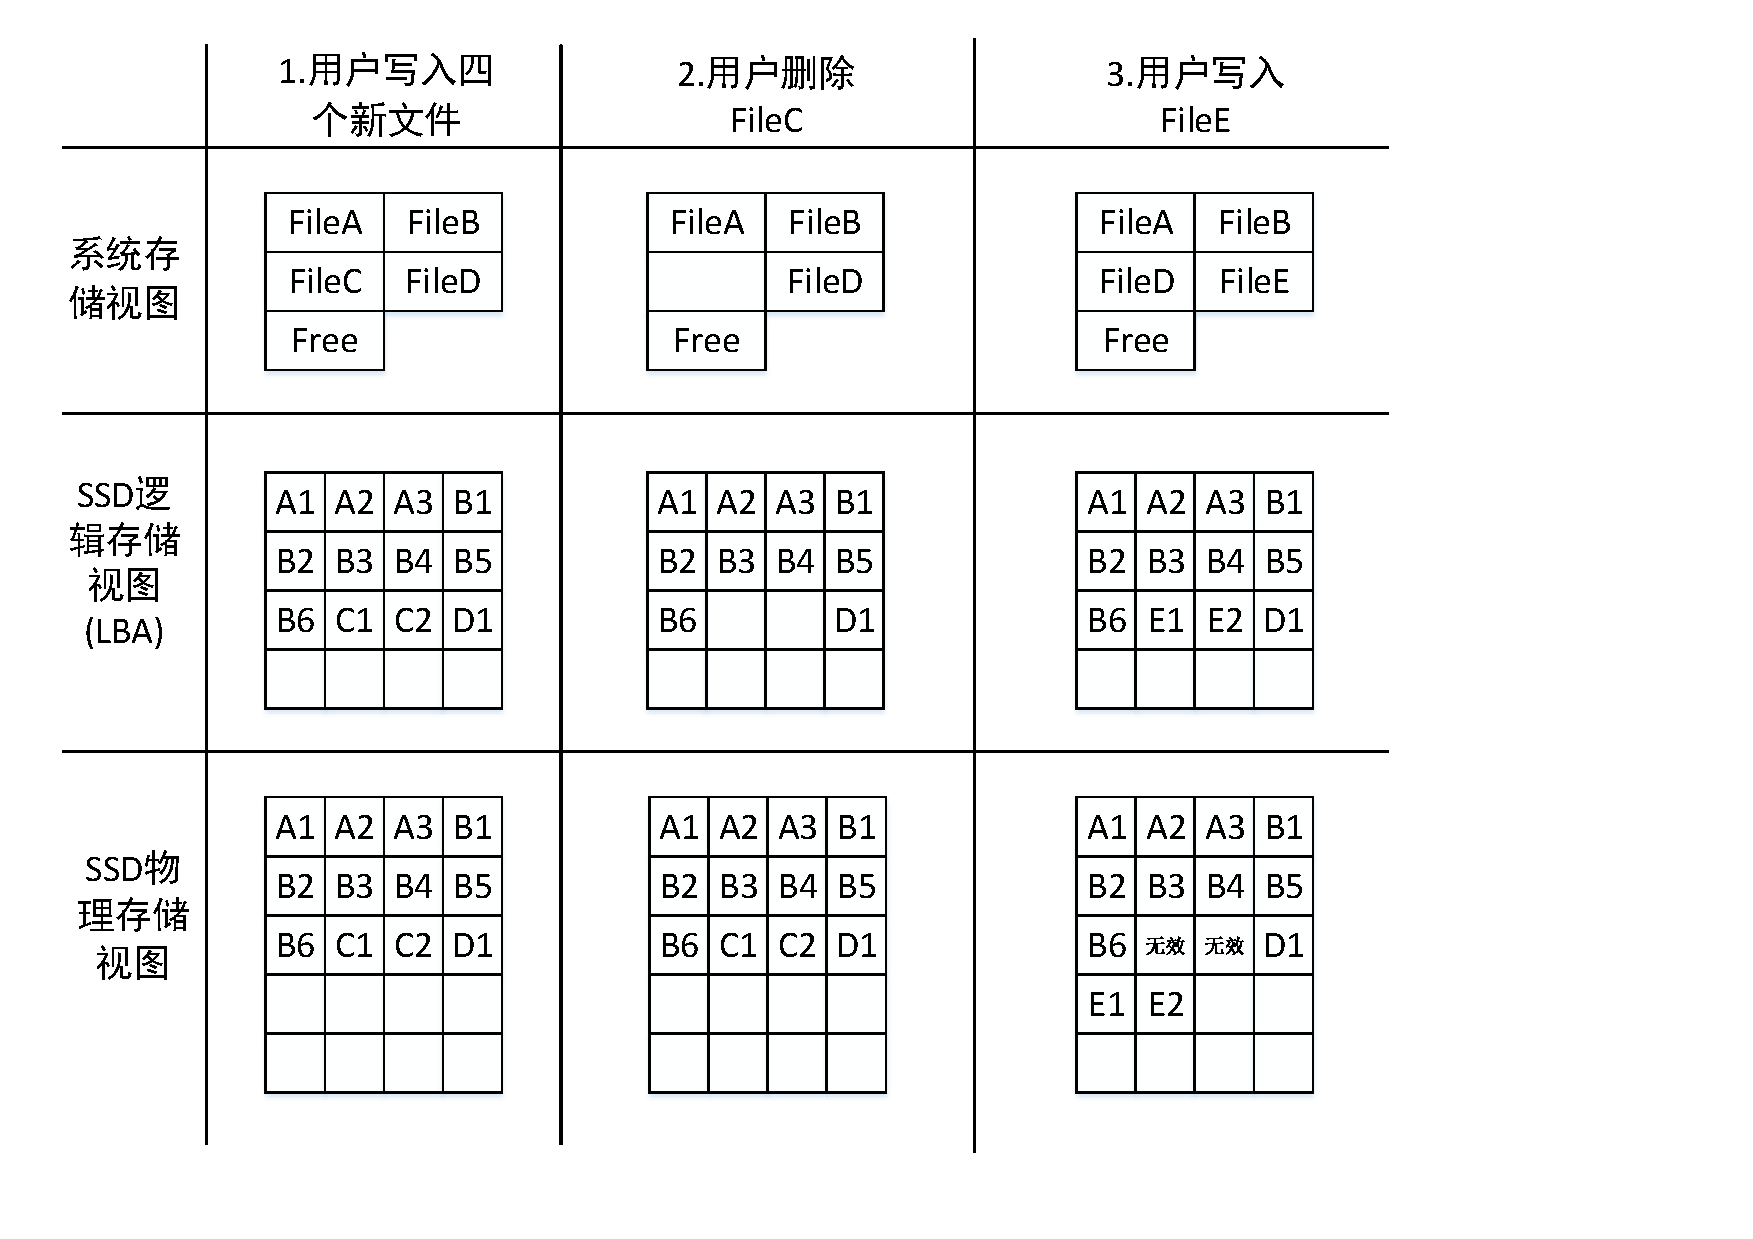
\includegraphics[width=4in]{Pics/fig-out-of-place.pdf}
\caption{固态盘异地更新}\label{fig:1}
\end{figure}
用户在文件系统上首先创建了FileA、FileB、FileC、FileD四个文件数据,反映到固态盘的逻辑块存储视图上的
数据,以及在固态盘物理介质上的数据块分别如\autoref{fig:1}所示。
当用户在系统中删除了文件FileC,但是在固态盘的逻辑存储地址和物理介质上,文件C的两个数据块C1、C2却没有删
除,也就是说,在用户删除文件数据的时候,数据依然存在。系统只是简单的返回一个“删除成功”的假象给用户。


第三步用户写入新的文件FileE时,虽然在固态盘逻辑块存储地址上,数据块C!,C2的位置被重新写入了新文件FileE
的存储地址,但是,在固态盘物理介质上,数据块E1、E2是写入到新的位置,而旧的数据块C1、C2只是被固态盘的垃
圾回收标记为“可回收”状态,真正被擦除的时机是不可控的。


从\autoref{fig:1}的三个简单操作可以发现,当用户删除了文件FileC之后,在物理介质上它的数据C1、C2在回收之
前,一直都没有真正地被删除掉,这就是固态盘“异地更新”的特性,利用固态盘的这个特性,攻击者使用一些安全工
具依然可以将被删掉的文件FileC恢复出来,这就造成了数据被窃取的风险。


怎样设计一套针对全闪存盘阵的安全删除方案,使得用户在物理介质上删除了元数据之后,存储的数据就能够保证安
全,这就就是我们课题要研究的重点。
\section{研究目的和意义}
在信息化时代,经济、军事领域对于数据的安全性要求是比较高的。由于关键信息的泄露,可能导致国家或者商业组织
非常重大的损失。在商业上,一个很小的文件泄露,可能导致公司上千万的经济损失;在国防安全领域,机密文件的泄
露,将对国家造成巨大的安全威胁。但是,目前来看,数据泄露的问题非常普遍,造成的问题层出不穷。具体而言,数
据泄露主要存在以下三个问题:


\textbf{(1) 在数据处理、传输、存储等中间过程中,数据可能被非法复制窃取。}
例如网络传输的邮件等可能会被第三方服务商缓存下来,这种不可预知的数据复制操作在互联网时代更加普遍。导
致一些企业用户纷纷兴建私有的数据中心,而不是接受公有云的服务,就是为了规避这类问题的风险。


\textbf{(2) 由于不同存储介质的特性不同,导致用户很难真正地删除数据。}虽然针对磁盘已存在很多安全工具,
如 O\&O SafeErase、DataWipe、BCwipe、HDDerase、SDelete、Secure Eraser 等\cite{safe-erase,secure-eraser,bcwipe} ,
这些工具基本都是根据针对普通磁盘的数据删除方法,使用特定数据对目标文件的逻辑页进行多次写入。其中有所不同的
仅仅是对哪些额外数据进行覆盖,例如文件系统元数据(如NTFS文件系统的MFT记录或日志)\cite{Huebner2006Data}、
系统虚拟内存文件、浏览器临时文件、空闲空间或已删除文件等等;或选用几种数据组合进行覆盖多少次。由于固态盘的异地
更新方法总是将写更新的数据写入到新的物理页,只是将过期的数据页标记为无效,这些过期的数据页无法从文件系统访问,
更无法查找和删除,而且,这些安全删除工具还会向用户报告数据擦除成功,使用户产生错觉,不仅不起作用,还可能带来更
大的数据泄露风险。另外,不同介质的存储设备在提供存储服务时,用户很难针对不同的设备使用不同的安全删除手段清除
数据,很有可能导致数据泄露。


\textbf{(3) 数据安全删除手段可能降低存储设备或系统的可靠性以及性能。}由于工艺制程的提高,固态盘的线宽
发展得更小,每单元存储的数据也越来越多,擦除寿命也变得更短\cite{Yaakobi2012Characterization,Shibata2012A}。\autoref{tab:1}
显示了闪存芯片从SLC发展到QLC的线宽、擦除寿命等数据。从表中可以看出,随着闪存芯片的发展,数据安全
删除的次数是不断下降的,由于基于闪存的存储设备或者系统集成了大量闪存芯片,即使是全新的固态盘也普遍
存在坏块,如果一块固态盘里有大量坏块,可能会影响其他更多的区块,导致芯片损坏\cite{Schroeder2016Flash}。
在新型非易失性存储器(Non-Volatile Memory,以下简称NVM)擦除寿命一定的情况下,如果删除特定数据,会增加擦除次数,
可能引入额外的擦除操作,也就可能影响基于新型 NVM 的存储设备或系统的可靠性。另一方面,在大数据时代,用户数据量巨大,
如果存储系统不加区分的实施数据安全删除操作,不但花费的时间长,而且会降低存储系统性能和可靠性。
因此,总体来说,对于数据安全的删除操作,会减少闪存芯片的剩余擦除次数,使其擦除寿命降
低,可能会导致坏块的增多,降低其性能,擦除操作过多更有可能导致不可预期的问题出现,影响存储设备的可靠性。

这些已经存在的风险说明,由于云环境下数据不可控和用户数据隐私安全的特点,需要研究出一套安全删除方案,这套方案面向新型
的闪存存储设备,需要对用户透明,并且缩小泄露用户敏感数据的时间窗口,同时保证系统的可靠性和高性能。这项研究不仅十分有意
义,而且由于研究仍处在起步阶段,这为升级我国计算机存储技术,甚至超越发达国家的存储技术水平,提供了一个很好的机会。
\begin{table}
\centering
\caption{SLC、MLC、TLC、QLC 四种闪存芯片的特性}\label{tab:1}
    \begin{tabular}{|*{5}{c|}}
\hline
    \multirow{2}{*}{闪存特性} & SLC & MLC & TLC & QLC \\
    & (Single-Level Cell) & (Multi-Level Cell) & (Triple-Level Cell) & (Quad-Level Cell) \\
\hline
    \textbf{存储单元模型} & 每单元一位数据 & 每单元两位数据 & 每单元三位数据 & 每单元四位数据 \\
\hline
    \textbf{速度} & 特别快 & 快 & 慢 & 很慢 \\
\hline
    \multirow{6}{*}{\textbf{擦除寿命}} & 10 万次 & 1万次 & 2500次 & 约500次 \\ %\multirow{2}{*}{约500次} \\
        & (5×nm) & (5×nm) & (5×nm) & \\ \cline{2-5}
    & 10 万次 & 5000次 & 1250次 & N/A \\%\multirow{2}{*}{N/A}  \\
        & (3×nm) & (3×nm) & (3×nm) &\\ \cline{2-5}
    & N/A & 3000次 & 750次 & N/A \\ %\multirow{2}{*}{N/A} \\
        & (2×nm) & (2×nm) & (2×nm) & \\ \hline
\end{tabular}
\end{table}


上述的三个问题说明了,一方面,数据的安全性需要做到安全删除,另一方面,研究基于固态盘阵的数据安全删除
是一项有意义的工作,国内外的研究工作都处于起步阶段,积极投身这个领域将会为我国的存储安全研究打开新的局面。

\section{国内外研究现状}
近几年来,针对固态盘的安全删除技术受到了广泛关注。在国内,包括华中科技大学、中南大学、武汉大学、西安电子
科技大学、中国科学院信息工程研究所、复旦大学等高等院校
和科研机构都开展了相关课题和理论的研究。在国外,美国的华盛顿大学、哥伦比亚大学、密歇根大学、纽卡斯尔大学
以及IBM、HP等实验室也积极地投身在安全删除领域的研究上。下面将分别介绍国内外的研究现状和部分研究成果。
\subsection{基于密码学意义上的安全删除}
数据在被加密存储之后,如何保证删除密钥数据,原来的数据就无法再被还原,成为新的难题。Perlman等人首次
提出了基于时间的数据安全删除方法,针对加密文件,如果密钥过期后数据即被删除,而且文件无法恢
复\cite{Perlman2005File}。受Perlman等人的启发,Tang等人设计出了FADE系统\cite{Tang2012Secure},该系统
使用公钥密码并使用简单的布尔操作来调整安全删除策略。但是FADE只支持一到两层的布尔表达,而且需要使用复杂的
公钥系统。Perlman等人还设计了Ephemerizer系统\cite{Perlman2005The,Tang2009Timed},该系统需要一个可信服务
器保存并管理由数据拥有者指定过期时间的解密密钥。Geambasu 等人给出了一个基于时间的数据可信删除方法的原
型 Vanish\cite{Geambasu2009Vanish},但Vanish容易受到跳跃攻击(hopping attack)和嗅探攻击(sniffing attack)\cite{Wolchok2010Defeating} 。
华中科技大学武汉光电国家实验室曾令仿等人提出了一种SafeVanish\cite{Zeng2010SafeVanish}方案,通过扩展密钥
等份长度的方法提高跳跃攻击的成本,并且引入公钥密码体制抵御嗅探攻击,显著改善了Vanish方案。Reimann等
人\cite{Reimann2012Timed}针对Vanish系统中当文件在 8 小时后需要被访问时,文件拥有者需要更新节点缓存中的
密钥部分问题,提出了将密钥分量分发到随机的网页中保存的改进方案,随着时间的改变,网页会改变存储内容或是
被删除。针对以Vanish为代表的加密方案存在的单个密钥加密全部数据不能对数据进行细粒度的管理等问题,武汉大学
王丽娜等人\cite{王丽娜2012一种适于云存储的数据确定性删除方法}提出了利用秘钥生成树,门限秘密共
享(threshold secret sharing)来组织和管理秘钥,同时利用分布式散列表(distributed hash table,DHT)周期
性地删除相关秘钥来实现安全删除。中南大学王国军等人改进了Vanish方案,除了将密钥分发到 DHT 网络中,还提取
部分密文并分发到DHT 网络中,从而更有效抵抗传统密码分析和暴力攻击\cite{Wang2010A}。西安电子科技大学马建峰
和中国科学院信息工程研究所李凤华所在课题组针对网络内容生命周期隐私保护问题,提出了面向网络内容隐私的基于
身份加密的安全自毁方案\cite{熊金波2014云计算环境中的组合文档模型及其访问控制方案,熊金波2014基于属性加密
的组合文档安全自毁方案,熊金波2014面向网络内容隐私的基于身份加密的安全自毁方案},这种方案基于身份的加密和
分布式Hash表(DHT)网络。这些方案更多的是偏向上层应用,在原型系统方面的实现和方法验证方面显得不足。

Mitra等人\cite{Mitra2006Secure}提出了通过反向索引来组织数据,其建立在加密且密钥数据能够被破坏的基础上,
从而可选择性地删除数据记录以及相关索引中的关键字。Castelluccia等人\cite{Castelluccia2011EphPub}提出了一
种EphPub协议阻止用户访问过期数据文件,是一种基于DNS及其缓存机制基础上的高效和鲁棒性协议。Backes等人设计
了一种X-pire系统\cite{Backes2011X},用户将加密的图像上传至社交网络,而将密钥外包给可信第三方管理。管理者
负责密钥的删除和更新、有效期延长缩短,用户查看加密图像时,管理者帮助其恢复密钥来解密。Cachin和Zhao等
人\cite{Cachin2013Policy,Zhao2015Gracewipe}通过基于加密的数据安全销毁的安全模型和安全定义,将图论(Graph)
、对称加密算法和门限密钥共享技术相结合以实现基于策略的安全数据销毁(policy-based secure deletion)。针对现有云
计设施,从可信计算的角度,张逢喆等设计的CloudVisor\cite{Zhang2011CloudVisor}和Dissolver\cite{张逢喆2011云计算中的数据隐私性保护与自我销毁}
系统实现数据隐私性保护与自我销毁。从云存储服务提供商对具有数据安全删除功能的存储系统需求的角度,华中科技大
学武汉光电国家实验室曾令仿已有研究SaDas\cite{Zeng2013SeDas}和CloudSky\cite{Zeng2015CloudSky},基于对象
存储技术,通过控制密钥生命周期的方法,结合基于属性加密(ABE),实现了可信第三方支持的具有数据安全删除功能
的存储系统。此外,Hao等人\cite{Feng2016Deleting}提出基于“信任,但要核查”的设计原则,通过应用加密允许
终端用户验证加密和删除两个重要功能的正确执行。

针对密钥从物理介质上“真正地”删除,这些方案涉及的研究都不是很深。另外,针对具有数据去重功能的存储系统,如何实施安全删除操作,
也是一个具有挑战性的问题。
\subsection{物理介质上数据安全删除}
面对这一问题,研究者有的提出了从物理损坏或者化学破坏的方式,这种方法不本方案不涉及相关研究。
M.Wei的一个研究\cite{Wei2011Reliably}表明:
\begin{enumerate}
\item 存储介质的内建命令通常能提供有效的数据擦除功能,但是并不能保证这些命令总是被制造商正确地实现
\item 将SSD的所有数据全部覆盖两次(在大部分情况下)能够有效地清除数据
\item 对于单个数据块删除而言,当前的SSD都存在不足之处
\end{enumerate}


因此,这一过程的实现并不一直是正确的,在有些情况,文件系统显示已被删除,而数据仍在设备中存在。Peterson等
人\cite{Peterson2005Secure}在数据块层使用全有或全无的转换技术(AONT)来实施安全删除,该方法通过AONT存储每
一个数据块,然后覆盖其中的一部分,这使得整个数据块不可用。2012年,Diesburg提出TrueErase\cite{Diesburg2012TrueErase},一
种类似于TRIM指令的功能,但是只针对属于某敏感文件的数据块。他们在文件系统和设备驱动之间增加了一个新的传输
通道。被修改的设备驱动一旦接受到被删除块的信息,使用其下层的接口就可以实现快速安全删除。TrueErase比TRIM更
有效,因为它可以只是安全擦除部分敏感块。TrueErase改造了存储管理层,全方位监控敏感文件的编辑和更新,并可彻
底删除敏感文件,前提是假设文件系统可以直接访问和操作物理闪存,所以其缺点是无法应用于普通固态盘。2016年,
Diesburg等人进一步改进了TrueErase的功能,对每一个文件使用了辅助的数据路径来提升数据安全删除的效果\cite{diesburg2016trueerase}。


总体来说,针对全闪存盘阵应用场景,目前研究都处在初始阶段,需要采用新的架构来保证数据的安全删除\cite{傅颖勋2013安全云存储系统与关键技术综述}。现
有研究偏向上层应用,并且越是接近上层系统越抽象,数据确定性删除就越困难\cite{Reardon2013SoK},也难以在存储
性能、计算开销和数据通信延迟方面达到很好的平衡\cite{李晖2014公共云存储服务数据安全及隐私保护技术综述}。另
外,现有研究缺乏从数据按需删除的角度,只针对敏感数据实施安全删除,从而并不改变普通用户的使用习惯,或根据
不同的安全级别需求采取“合理”的数据安全删除策略。
\section{本文的研究内容}
本研究旨在提供一种基于闪存盘组成的阵列的数据安全删除方案。通过对数据进行冗余加密,保障数据安全存储,即高
可靠性和高安全性。一方面,采用了非对称加密算法、群域运算保障数据可靠性;另一方面,在编码前引入加密的方式
增强数据隐私保护,利用冗余编码的特性结合弱密钥思想,对数据的删除不再需要对整个数据进行覆盖写,而是删除部
分数据块,破坏数据完整性或者密钥完整性,使数据无法正常读取。即使攻击者得到数据,也不能获取明文,达到数据
安全删除的目的。本研究在保证数据安全存储的同时,降低了对固态盘阵列的读写访问,相当于延长了固态盘的使用寿命。
